%%%%%%%%%%%%%%%%%%%%%%%%%%%%%%%%%%%%%%%%%%%%%%%%%%%%%%%%%%
%   Vorlage von:
%
%   Prof. Dr. Bernhard Drabant
%   Prof. Dr. Dennis Pfisterer
%   Prof. Dr. Julian Reichwald
%
%%%%%%%%%%%%%%%%%%%%%%%%%%%%%%%%%%%%%%%%%%%%%%%%%%%%%%%%%%

%%%%%%%%%%%%%%%%%%%%%%%%%%%%%%%%%%%%%%%%%%%%%%%%%%%%%%%%%%
%	ANLEITUNG: 
%
%   1. Ersetzen Sie firmenlogo.jpg im Verzeichnis img
%   2. Passen Sie alle Stellen im Dokument an, die mit 
%      @stud markiert sind
%
%%%%%%%%%%%%%%%%%%%%%%%%%%%%%%%%%%%%%%%%%%%%%%%%%%%%%%%%%%

%%%%%%%%%%%%%%%%%%%%%%%%%%%%%%%%%%%%%%%%%%%%%%%%%%%%%%%%%%
%	ACHTUNG: 
%
%   Für das Erstellen des Literaturverzeichnisses wird das 
%   modernere Paket biblatex in Kombination mit biber 
%   verwendet -- nicht mehr das ältere BibTex!
%   Bitte stellen Sie ggf. Ihre TeX-Umgebung entsprechend 
%   ein (z.B. TeXStudio: Einstellungen --> Erzeugen --> 
%   Standard Bibliographieprogramm: biber)
%
%%%%%%%%%%%%%%%%%%%%%%%%%%%%%%%%%%%%%%%%%%%%%%%%%%%%%%%%%%

\documentclass[fontsize=12pt,BCOR=5mm,DIV=12,
               parskip=half,
               listof=entryprefix,paper=a4,toc=bibliography,toc=listof,pointlessnumbers,ngerman
               %,headinclude=on,footinclude=off,
               %,plainheadtopline=false,plainheadsepline=false,plainfootsepline=false,plainfootbotline=false
               ]{scrreprt}
               
\makeindex

% (!!) Elementare Pakete, Konfigurationen und Definitionen werden geladen
% !TEX root =  master.tex
%      HYPERREF

%%%%%%%%%%%%%%%%%%%%%%%%%%%%%%%%%%%%%%%%%%%%%%%%%%%%%%%%%%
%	ANLEITUNG: 
%
% Passen Sie alle Stellen im Dokument an, die mit 
% @stud markiert sind
%
%%%%%%%%%%%%%%%%%%%%%%%%%%%%%%%%%%%%%%%%%%%%%%%%%%%%%%%%%%

\usepackage{makeidx}         % allows index generation
\usepackage{listings}	%Format Listings properly
\usepackage{lipsum}    %Blindtext
\usepackage{graphicx} % use various graphics formats
\usepackage[german]{varioref} 	% nicer references \vref
\usepackage{caption}	%better Captions
\usepackage{booktabs} %nicer Tabs
\usepackage{array}
\usepackage{chngcntr}
\usepackage[hidelinks=true]{hyperref} % keine roten Markierungen bei Links
\usepackage{fnpct} % Correct superscripts 
\usepackage[T1]{fontenc}
\usepackage[utf8]{inputenc}
\usepackage{calc} % Used for extra space below footsepline
\usepackage{acronym}
\usepackage{algorithm}
\usepackage{algpseudocode}
\usepackage{setspace}
\usepackage{wrapfig}
\usepackage{tabularx}

%
% @stud
%
%	FONT SELECTION: Entweder 1) Latin Modern oder 2) Times / Helvetica
\usepackage{lmodern}             % 1) Latin modern font
%\usepackage{mathptmx}           % 2) Helvetica / Times New Roman fonts (2 lines)
%\usepackage[scaled=.92]{helvet} % 2) Helvetica / Times New Roman fonts (2 lines)

%
% @stud
%
%	LANGUAGE SETTINGS
\usepackage[ngerman]{babel} 	        % german language
\usepackage[german=quotes]{csquotes} 	% correct quoting using \enquote{}
%\usepackage[english]{babel}          % english language
%\usepackage{csquotes} 	              % correct quoting using \enquote{}

%
% @stud
%
% Uncomment the following lines to support hard URL breaks in bibliography 
%\apptocmd{\UrlBreaks}{\do\f\do\m}{}{}
%\setcounter{biburllcpenalty}{9000}% Kleinbuchstaben
%\setcounter{biburlucpenalty}{9000}% Großbuchstaben

%
% @stud
%
%	FOOTNOTES: Count footnotes over chapters
%1 \counterwithout{footnote}{chapter}

%	ACRONYMS
\makeatletter
\@ifpackagelater{acronym}{2015/03/20}
{\renewcommand*{\aclabelfont}[1]{\textbf{{\acsfont{#1}}}}}{}
\makeatother

%	LISTINGS
\renewcommand{\lstlistingname}{Quelltext} 
\renewcommand{\lstlistlistingname}{Quelltextverzeichnis}
\lstset{numbers=left,
	numberstyle=\tiny,
	captionpos=b,
	basicstyle=\ttfamily\small}

%	ALGORITHMS
\renewcommand{\listalgorithmname}{Algorithmenverzeichnis }
\floatname{algorithm}{Algorithmus}

%		PAGE HEADER / FOOTER
%	    Warning: There are some redefinitions throughout the master.tex-file!  DON'T CHANGE THESE REDEFINITIONS!
\RequirePackage[automark]{scrlayer-scrpage}
%alternatively with separation lines: \RequirePackage[automark,headsepline,footsepline]{scrlayer-scrpage}

%\renewcommand*{\pnumfont}{\upshape\sffamily}
%\renewcommand*{\headfont}{\upshape\sffamily}
%\renewcommand*{\footfont}{\upshape\sffamily}

\renewcommand{\chaptermarkformat}{}
\RedeclareSectionCommand[beforeskip=0pt]{chapter}
\clearscrheadfoot

%\ifoot[\rule{0pt}{\ht\strutbox+\dp\strutbox}DHBW Mannheim]{\rule{0pt}{\ht\strutbox+\dp\strutbox}DHBW Mannheim}
\ofoot[\rule{0pt}{\ht\strutbox+\dp\strutbox}\pagemark]{\rule{0pt}{\ht\strutbox+\dp\strutbox}\pagemark}
\ohead{\headmark}

\newcommand{\TitelDerArbeit}[1]{\def\DerTitelDerArbeit{#1}\hypersetup{pdftitle={#1}}}
\newcommand{\AutorDerArbeit}[1]{\def\DerAutorDerArbeit{#1}\hypersetup{pdfauthor={#1}}}
\newcommand{\Firma}[1]{\def\DerNameDerFirma{#1}}
\newcommand{\Kurs}[1]{\def\DieKursbezeichnung{#1}}
\newcommand{\Abteilung}[1]{\def\DerNameDerAbteilung{#1}}
\newcommand{\Studiengangsleiter}[1]{\def\DerStudiengangsleiter{#1}}
\newcommand{\WissBetreuer}[1]{\def\DerWissBetreuer{#1}}
\newcommand{\FirmenBetreuer}[1]{\def\DerFirmenBetreuer{#1}}
\newcommand{\Bearbeitungszeitraum}[1]{\def\DerBearbeitungszeitraum{#1}}
\newcommand{\Abgabedatum}[1]{\def\DasAbgabedatum{#1}}
\newcommand{\Matrikelnummer}[1]{\def\DieMatrikelnummer{#1}}
\newcommand{\Studienrichtung}[1]{\def\DieStudienrichtung{#1}}
\newcommand{\ArtDerArbeit}[1]{\def\DieArtDerArbeit{#1}}
\newcommand{\Literaturverzeichnis}{Literaturverzeichnis}

\usepackage[backend=biber, autocite=footnote, style=authoryear, dashed=false]{biblatex}
\DefineBibliographyStrings{ngerman}{  %Change u.a. to et al. (german only!)
	andothers = {{et\,al\adddot}},
}
\setlength{\bibparsep}{\parskip}		%add some space between biblatex entries in the bibliography
\addbibresource{bibliography.bib}	%Add file bibliography.bib as biblatex resource
\usepackage{chngcntr}
\counterwithout{footnote}{chapter}


\newcommand{\setTitlepage}{
	% !TEX root =  master.tex
\begin{titlepage}
	\begin{center}
		
\includegraphics[width=8cm]{\imagedir/logo.jpg}	
	\end{center}
	\vspace{2em}
	%\sffamily
	\begin{center}
		{\textsf{\large Duale Hochschule Baden-W\"urttemberg Mannheim}}\\[4em]
		{\textsf{\textbf{\large{\DieArtDerArbeit}arbeit}}}\\[6mm]
		{\textsf{\textbf{\Large{}\DerTitelDerArbeit}}} \\[1.5cm]
		{\textsf{\textbf{\large{}Studiengang Wirtschaftsinformatik}}\\[6mm]
		\textsf{\textbf{Studienrichtung \DieStudienrichtung}}}\\[6mm]
		\textsf{Kurs: \DieKursbezeichnung} \\[3cm]
		\begin{center}
			\begin{table}[h]
				\centering
				\begin{tabular}{c}
					Aaron Schweig \\
					Troy Kessler  \\
					Matthias Vonend  \\
					Michael Angermeier \\
					Patrick Mischka \\
					Jan Grübener \\
				\end{tabular}
			\end{table}
		\end{center}

		% \begin{minipage}{\textwidth}
		% 	\begin{tabbing}
		% 		Bearbeitungszeitraum: \hspace{0.85cm}\=\kill
		% 		% TODO: Verfasser
		% 		Kurs: \> \DieKursbezeichnung \\[1.5mm]
		% 		Bearbeitungszeitraum: \> \DerBearbeitungszeitraum\\[1.5mm]
		% %		alternativ:\\[1.5mm]
		% %		Eingereicht: \> \DasAbgabedatum	
		% 	\end{tabbing}
		% \end{minipage}
	\end{center}
\end{titlepage}
	\pagenumbering{roman} % Römische Seitennummerierung
	\normalfont	
}

%
% @stud
%
\newcommand{\settingLists}{
	%	Inhaltsverzeichnis
	\tableofcontents
	%	Abbildungsverzeichnis
	\listoffigures
	%	Tabellenverzeichnis
	\listoftables
	%	Listingsverzeichnis / Quelltextverzeichnis
	\lstlistoflistings
	% Algorithmenverzeichnis
	% \listofalgorithms
}

\newcommand{\initializeText}{
	\clearpage
	\ihead{\chaptername~\thechapter} % Neue Header-Definition
	\pagenumbering{arabic}           % Arabische Seitenzahlen
}

\newcommand{\initializeBibliography}{
	\ihead{}
	\printbibliography[title=\Literaturverzeichnis] 
	\cleardoublepage
}

\newcommand{\initializeAppendix}{
	\appendix
	\ihead{\appendixname~\thechapter}
}

\newcommand{\setword}[2]{%
  \phantomsection
  #1\def\@currentlabel{\unexpanded{#1}}\label{#2}%
}


\usepackage{color}

\definecolor{mygreen}{rgb}{0,0.6,0}
\definecolor{mygray}{rgb}{0.5,0.5,0.5}
\definecolor{mymauve}{rgb}{0.58,0,0.82}

\lstset{ 
  backgroundcolor=\color{white},
  breakatwhitespace=false,
  breaklines=true,
  captionpos=b,
  commentstyle=\color{mygreen},
  extendedchars=true,
  frame=single,
  keepspaces=false,
  keywordstyle=\color{blue},
  language=Java,
  numbers=left,
  numbersep=5pt,
  numberstyle=\color{mygray},
  rulecolor=\color{black},
  showspaces=false,
  showstringspaces=false,
  showtabs=false,
  stepnumber=2,
  stringstyle=\color{mymauve},
  tabsize=2,
  title=\lstname,
  basicstyle=\scriptsize
}

\usepackage{xspace}
% \usepackage{pifont}

\usepackage{tikz}
\newcounter{barcount}
\newenvironment{barchart}[1]{ % The only parameter is the maximum bar width, in cm
	\newcommand{\barwidth}{0.35}
	\newcommand{\barsep}{0.55}

	% Command to add a bar to the bar chart
	\newcommand{\baritem}[2]{ % The first argument is the bar label and the second is the percentage the current bar should take up of the total width
		\pgfmathparse{##2}
		\let\perc\pgfmathresult

		\pgfmathparse{#1}
		\let\barsize\pgfmathresult

		\pgfmathparse{\barsize*##2/5}
		\let\barone\pgfmathresult

		\pgfmathparse{(\barwidth*\thebarcount)+(\barsep*\thebarcount)}
		\let\barx\pgfmathresult

		\filldraw[fill=none, draw=black!] (0,-\barx) rectangle (5,-\barx-\barwidth);
		\filldraw[fill=black!90, draw=black!90] (0,-\barx) rectangle (\barone,-\barx-\barwidth);

		\node [label=180:{\textcolor{black}{##1: ##2/5}}] at (0,-\barx-0.175) {};
		\addtocounter{barcount}{1}
	}

	\newcommand{\baritemNL}[2]{ % The first argument is the bar label and the second is the percentage the current bar should take up of the total width
		\pgfmathparse{##2}
		\let\perc\pgfmathresult

		\pgfmathparse{#1}
		\let\barsize\pgfmathresult

		\pgfmathparse{\barsize*##2/5}
		\let\barone\pgfmathresult

		\pgfmathparse{(\barwidth*\thebarcount)+(\barsep*\thebarcount)}
		\let\barx\pgfmathresult

		\filldraw[fill=none, draw=black!] (0,-\barx) rectangle (5,-\barx-\barwidth);
		\filldraw[fill=black!90, draw=black!90] (0,-\barx) rectangle (\barone,-\barx-\barwidth);

		\node [label=180:{}] at (0,-\barx) {};
		\addtocounter{barcount}{1}
	}

	\begin{tikzpicture}
	\setcounter{barcount}{0}
}{
	\end{tikzpicture}
	\vspace{0.3cm}
}


%%%%%%%%%%%%%%%%%%%%%%%%%%%%
%
% @stud
%
%	SCHRIFTART (Schrift mit oder ohne Serifen im gesamten Text) 
%
% mit Serifen
%\addtokomafont{disposition}{\rmfamily}
%\renewcommand*{\familydefault}{\rmdefault}
%
% ohne Serifen (default)
%\addtokomafont{disposition}{\sffamily}
%
%%%%%%%%%%%%%%%%%%%%%%%%%%%%

%%%%%%%%%%%%%%%%%%%%%%%%%%%%
%
% @stud
%
% PERSÖNLICHE ANGABEN (BITTE VOLLSTÄNDIG EINGEBEN zwischen den Klammern: {...})
%
\ArtDerArbeit{Studien} % "Bachelor" oder "Projekt" wählen
\TitelDerArbeit{Projektrealisierung - Simulation}
\Kurs{WWI18SEA/C}
\Studienrichtung{Software Engineering}

%%%%%%%%%%%%%%%%%%%%%%%%%%%%

%%%%%%%%%%%%%%%%%%%%%%%%%%%%
%
% @stud
%
%	BIBLIOGRAPHY (@stud: Bibliographie-Stil wählen - Position und Indizierung)
%
% Auswahl zwischen: IEEE Style, ALPHABETIC Style, HARVARD Style, AUTHOR-YEAR Style 
%
% (oder eigenen zulässigen Stil wählen) 
%

% Position des Zitats
%
\newcommand{\position}{inline} 
%\newcommand{\position}{footnote}

% Indizierung des Zitats
%
% 1) NUMERIC Style - e. g. [12]
\newcommand{\indextype}{numeric} 
%
% 2) ALPHABETIC Style - e. g. [AB12]
%\newcommand{\indextype}{alphabetic} 
%
% 3) IEEE Style - numeric kind of style 
%\newcommand{\indextype}{ieee} 
%
% 4) HARVARD Style 
%\newcommand{\indextype}{apa} 
%
% 5) CHICAGO Style 
%\newcommand{\indextype}{authoryear}
%
%%%%%%%%%%%%%%%%%%%%%%%%%%%%

\renewcommand*{\familydefault}{\sfdefault}

% \usepackage[backend=biber, autocite=\position, style=\indextype]{biblatex} 	

% \settingBibFootnoteCite

\newcommand{\abs}{\par\vskip 0.2cm\goodbreak\noindent}
\newcommand{\nl}{\par\noindent}
\newcommand{\mcl}[1]{\mathcal{#1}}
\newcommand{\nowrite}[1]{}
\newcommand{\NN}{{\mathbb N}}

\newcommand{\imagedir}{img}

\makeindex

\begin{document}

\setTitlepage

%%%%%%%%%%%%%%%%%%%%%%%%%%%%%%%%%%%%%%%%%%%%%%%%%%%%%%%%%%%%%%%%%%%%%%%%%%%%%%%%%%%%%%%%%%
% KAPITEL UND ANHÄNGE
%
% @stud:
%   - nicht benötigte: auskommentieren/löschen
%   - neue: bei Bedarf hinzufügen mittels input-Kommando an entsprechender Stelle einfügen
%%%%%%%%%%%%%%%%%%%%%%%%%%%%%%%%%%%%%%%%%%%%%%%%%%%%%%%%%%%%%%%%%%%%%%%%%%%%%%%%%%%%%%%%%%

%%%%%%%%%%%%%%%%%%%%%%%%%%%%%%%%%%%
% EHRENWÖRTLICHE ERKLÄRUNG
%
% @stud: ewerkl.tex bearbeiten
%
% \input{ewerkl} 
%%%%%%%%%%%%%%%%%%%%%%%%%%%%%%%%%%%

%%%%%%%%%%%%%%%%%%%%%%%%%%%%%%%%%%%
% SPERRVERMERK
%
% @stud: nondisclosurenotice.tex bearbeiten
%
% \input{nondisclosurenotice} 
%%%%%%%%%%%%%%%%%%%%%%%%%%%%%%%%%%%

%%%%%%%%%%%%%%%%%%%%%%%%%%%%%%%%%%%
%	KURZFASSUNG
%
% @stud: acknowledge.tex bearbeiten
%
% \input{acknowledge} 
%%%%%%%%%%%%%%%%%%%%%%%%%%%%%%%%%%%

%%%%%%%%%%%%%%%%%%%%%%%%%%%%%%%%%%%
%	KURZFASSUNG
%
% @stud: abstract.tex bearbeiten
%
% % !TEX root =  master.tex
\chapter*{Kurzfassung}

 
%%%%%%%%%%%%%%%%%%%%%%%%%%%%%%%%%%%

%%%%%%%%%%%%%%%%%%%%%%%%%%%%%%%%%%%
% VERZEICHNISSE
%
% @stud: ggf. nicht benötigte Verzeichnisse auskommentieren/löschen in Def. von \settingLists in config.tex
%
\settingLists
%%%%%%%%%%%%%%%%%%%%%%%%%%%%%%%%%%%

%%%%%%%%%%%%%%%%%%%%%%%%%%%%%%%%%%%
% ABKÜRZUNGSVERZEICHNIS
%
% @stud: acronyms.tex bearbeiten
%
% !TEX root =  master.tex
\clearpage
\chapter*{Abkürzungsverzeichnis}	
\addcontentsline{toc}{chapter}{Abkürzungsverzeichnis}

\begin{acronym}[XXXXXXX]
    \acro{API}[Application Programming Interface]{API}

\end{acronym} 
%%%%%%%%%%%%%%%%%%%%%%%%%%%%%%%%%%%

\initializeText
\onehalfspacing

%%%%%%%%%%%%%%%%%%%%%%%%%%%%%%%%%%%
% KAPITEL
%
% @stud: einzelne Kapitel bearbeiten und eigene Kapitel hier einfügen
%
% Einleitung
% !TEX root =  master.tex
\chapter{Einleitung}
\section{Motivation und Zielsetzung}

	
	Im Rahmen der Vorlesung \enquote{Projekt} des WWI18SEAC Kurses ist eine fiktionale Börse exemplarisch als Projekt mit unterschiedlichen Projektteams realisiert worden. Die verschiedenen Funktionen des Wertpapierhandels liegen in dem Verantwortungsbereich von unterschiedlichen Teams. Ein Vorlesungsfokus stellt die Koordination und Integration der Gruppen untereinander dar, wobei auch auf fachliche Korrektheit der behandelten Sachverhalte zu achten ist.\\
	Diese Arbeit stellt die Tätigkeiten des \enquote{Simulation}-Teams dar. Das Ziel der Simulation sind realistische Marktsituationen für unterschiedliche Marktpapiere darzustellen. Simulierte Kursverläufe sollen realitätsnah verschiedene Ordertypen aufweisen und Preisentwicklungen in verschiedenen Ausmaßen nach beinhalten. \\
	Andere Projektteams realisieren die Funktionalitäten von der zentralen Börse, von einem Privatbroker und von einem Geschäftsbroker. Die simulierten Kurse reagieren auf den Handel von unterschiedlichen Handelsteilnehmer, was für ein realistisches Marktverhalten notwendig ist.\\
	Als Grundlage für Kursentwicklungen dienen Szenarien, die dem Kursverlauf der SAP-Aktie aus den letzten zwei Jahren bei der entnommen wurden. Hierbei wurde auf Kursdaten der NASDAQ-Börse zurückgegriffen, da diese umfänglich und kostenfrei zur Verfügung stehen, was im Gegensatz bei den deutschen Handelsplätzen nicht der Fall war. Die entnommen Kursverläufe richten sich an unterschiedlichen Ereignissen, um ein möglichst breites Spektrum von Marktverhalten abzudecken.\\
	Das Ziel der Vorlesung ist die Zusammenarbeit von unterschiedlichen Teams innerhalb eines Projekts mit einem gemeinsamen Projektergebnis zu vermitteln und Grundlegende Verhaltensweisen aufzuzeigen. Das Ziel des Projektes selbst ist, unter Beachtung der fachlichen Korrektheit des Börsenhandels, eine funktionierende Börsenplattform zu realisieren.


\section{Aufbau der Arbeit}

	% Theorie
	% Fama
	% Szenarien
	
	Die Arbeit beginnt mit den theoretischen Ansätzen zur Erstellung der unterschiedlichen Kursverläufe. Erste Überlegungen beschäftigten sich mit dem Fama-French-Dreifaktorenmodell. Bei diesem Modell wird eine Aktienrendite vorhergesagt, welche mithilfe von Marktfaktoren und unterschiedlichen Unternehmens- und Kurseigenschaften berechnet wird.\\
	Diese Berechnung war im Rahmen der Simulation schwierig umzusetzen, wodurch die Entscheidung gefallen ist, diesen Ansatz zu verwerfen. Das Fama-French-Modell benötigt zur Berechnung den Unternehmensbuchwert, welcher über die Bilanz von Aktiengesellschaften auszuweisen ist. Diesen realistisch zu simulieren stellte die größte Hürde bei einer Verwendung des Fama-French-Modells dar. Als einfacher umzusetzende Alternative ist ein Szenario Ansatz verfolgt, welcher mit vordefinierten Daten umgesetzt wird. Historische Daten sind der NASDAQ-Börse entnommen und die ausgewählten Markttage orientieren sich an unterschiedlichen realen Marktsituationen. Diese variieren von einem Feiertag (an dem halbtags an der NASDAQ gehandelt wird) bis hin zu einer desaströsen Bilanzveröffentlichung, durch welche ein Massenverkauf und ein damit einhergehenden Kurseinbruch ausgelöst wird.
	
	% Anforderungsanalyse
	% Funktionale Anforderungen
	% Nicht Funktionale Anforderungen
	% Begrenzung von theoretischen Grundlagen
	% Anforderungen an andere Teams
	
	Im darauf folgenden Kapitel wird aus den bereits genannten thematischen Rahmenbedingungen Anforderungen an die Simulation abgeleitet. Diese sind zwischen funktionalen und nicht-funktionalen Anforderungen zu unterscheiden. Folglich werden die theoretischen Ansätze in Verbindung mit den herausgearbeiteten Anforderungen kritisch betrachtet und gegebenenfalls eingeschränkt. Als Abschluss dieses Kapitels sind Anforderungen an andere Projektteams dokumentiert.
	
	% Konzeption
	
	Im Rahmen der Konzeption wird die technischen Umsetzung näher erläutert und konkrete Vorgehensweisen dargestellt. Als Grundlage für die Konzeption dienen die bereits dokumentierten Anforderungen aus dem vorherigen Kapitel. Die entsprechende Konzeption soll funktionale und nicht-funktionale Anforderungen realisieren können und auf der anderen Seite Schnittstellen bereitstellen, um die Inhalte der Anforderungen an anderen Teams integrieren zu können. Hauptbestandteile sind das Vorgehen bei unterschiedlichen Szenarios und wie aus diesen konkrete Orders entstehen. Des Weiteren wird konkret Bezug darauf genommen, wie der Einfluss von anderen Marktteilnehmern die Orders des simulierten Marktes beeinflussen.
	
	Darauffolgend ist die konkrete Implementierung dokumentiert, wobei die verwendeten Schnittstellen eine besondere Bedeutung haben.\\
	Als inhaltlich letztes Kapitel ist das Nutzerhandbuch ein Anleitung zur Verwendung des entwickelten Codes, um die gezeigten Funktionalitäten nachvollziehen zu können, und die Simulation in Verbindung mit den anderen Projektbestandteilen auch von Dritten rekonstruiert werden kann.
	
	Das abschließende Kapitel dieser Dokumentation stellt die Zusammenfassung dar, die einen Überblick über die geleisteten Leistungen bringen soll und auf die Projektergebnisse kritisch Bezug nimmt.
	

% mehrere Grundlagen- und Forschungs-Kapitel
\input{chapters/theorie.tex}
% !TEX root =  ../master.tex
\chapter{Anforderungsanalyse}

In diesem Kapitel werden zuerst die funktionalen und nicht-funktionalen Anforderungen der Simulation erläutert. Anschließend werden diese Anforderungen übersichtlich zusammengefasst. Im Anschluss werden kurz die Anforderungen aus unserer Sicht zu den anderen Teilprojekten erläutert.
\section{Funktionale Anforderungen}
	\begin{itemize}
		\item Anmeldung: \\
			Damit das Marktgeschehen nicht durch jede beliebige Person beeinflusst werden kann, soll die Anwendung durch ein Login geschützt werden. So können nur dedizierte Personen Szenarien auswählen und wichtige Marktfaktoren beeinflussen. Denkbar wäre hierdurch auch das Verteilen von Berechtigungen.
			Beispielsweise wäre es möglich, lesende Operationen wie das gehandelte Volumen für alle einsehbar zu machen, während schreibende Operationen, die das Marktgeschehen beeinflussen könnten, nur ausgewählte Personen tätigen können.
		
		\item Auswahl vordefinierter Szenarien: \\
			Es soll eine Liste an vordefinierten Szenarien geben. Diese Szenarien können bestimmte Ereignisse sein, wie der Rücktritt einzelner Vorstandsmitglieder, auf die der Markt in einem vorher definierten Rahmen reagiert. Diese Reaktion soll automatisch mit dem Beginn des nächsten Szenarios durch die Simulation auf den Markt übertragen werden.
			
		\item Übersicht über die gerade gehandelten Trades: \\
			Es sollte eine grafische Übersicht geben, die einen Überblick über das durch die Simulation gehandelten Volumina und Preise verschafft.
			So soll ein besserer Einblick über die aktuelle Simulationsaktivität gegeben werden.
			
		\item Kommunikation von Events: \\
			Bestimmte Ereignisse beeinflussen das Marktgeschehen. Damit Privatkunden und Unternehmen, die an der Börse handeln, entsprechend reagieren können, müssen sie über solche Ereignisse aktiv informiert werden. Ob und wie sie auf diese Nachrichten reagieren bleibt ihnen selbst überlassen.
			
		\item Reaktion auf Marktgeschehen durch Privat- und Unternehmensbroker: \\
			Um die Simulation möglichst realistisch zu gestalten, muss auch das Verhalten und die Trades der anderen Marktteilnehmer berücksichtigt werden. Wichtig ist hier jedoch, dass nicht eine einzelne Transaktion eines Privatkunden schon die Marktpreise zum Schwanken bringt.
			Stattdessen sollen Transaktionen erst eine kritische Masse erreichen müssen, um wirklich auf dem Markt ins Gewicht zu fallen. 
			
		\item Anpassung der Dauer eines Szenarien: \\
			Um das schnelle Testen von Anlagestrategien zu ermöglichen, soll die Länge der Szenarien skalierbar sein.
	\end{itemize}
	
\section{Nicht-Funktionale Anforderungen}
		\begin{itemize}
		\item Geschwindigkeit: \\
			Für Nutzer ist die Geschwindigkeit besonders wichtig. Lang ladende Anwendungen sind nervig in der Benutzung und demotivieren die Nutzung der Anwendung. Über lange Ladezeiten beschweren sich in einer Umfrage mehr als 70\%, wobei 25\% aller Nutzer bereits bei 4 Sekunden die Seite verlassen. Aus diesem Grund sollte die Ladezeit gering gehalten werden.
			
		\item Skalierbarkeit: \\
			Um das bereits angesprochene hohe Ordervolumen zu realisieren, muss die Anwendung gut skalieren können.
			Bei zunehmender Zahl der Transaktionen oder Wertpapieren darf die Reaktion und die Performance der Anwendung nicht beeinträchtigt werden. 
	\end{itemize}

\section{Zusammenfassung}
	\begin{table}[ht!]
		\centering
		\begin{tabularx}{.8\textwidth}{l|X}
			Nr.     & Beschreibung                              \\\hline
			F1      & Am System soll eine Anmeldung möglich sein                  \\
			F2		& Es soll eine Szenarienauswahl geben \\
			F3      & Nutzer sollen eine Übersicht über die aktuelle Simulationsaktivität bekommen  \\
			F4      & Events, die das Marktgeschehen beeinflussen sollen aktiv kommuniziert werden  \\
			F5      & Es soll auf das Marktgeschehen durch andere Privat- und Unternehmensbroker reagiert werden  \\
			F6      & Die Zeiteinheiten und somit die Dauer eines Szenarien sollte angepasst werden können  \\\hline
			NF1     & Anwendung lädt schnell                    \\
			NF2     & Die Anwendung ist skalierbar                \\
		\end{tabularx}
		\caption{Zusammengefasste Anforderungen}
		\label{tab:anforderungen}
	\end{table}



\section{Anforderungen an andere Teams}\label{sec:otherTeams}
	Im Falle der Simulation bestehen keine Abhängigkeiten zu anderen Brokern. Bei den Privatkunden und Unternehmenskunden handelt es sich auch um Broker.
	Diese kaufen und verkaufen an der Börse Wertpapiere. Genauso wie bei der Simulation handelt es sich damit um Broker bzw. Clients der Börse, die sich lediglich in ihrer Zielgruppe und dem Zweck unterscheiden. Somit bleibt als einzige Schnittelle die Börse. Dabei wurden folgende Anforderungen aufgestellt:
	
	\textbf{GET-Requests}
		\begin{itemize}
			\item aktueller Preis eines Wertpapiers
			\item im Handel befindliche Wertpapiere
		\end{itemize}
	\textbf{POST-Requests}
		\begin{itemize}
			\item Order einstellen
		\end{itemize}
	\textbf{Aktive Benachrichtigungen}
		\begin{itemize}
			\item Buchung der Order
			\item Handel unterbrochen
		\end{itemize}

% !TEX root =  ../master.tex
\chapter{Konzeption}
\section{Herleitung und Betrachtung verschiedener Szenarien}\label{sec:szenarien}
Damit mit der Simulation der Markt möglich genau widergespiegelt werden kann, steht zunächst die Frage offen,
wie ein typischer Handelstag an der Börse aussieht. Um dies analysieren zu können, wird ein Aktienkurs betrachetet, 
der in den letzten Jahren meistens sehr stabil war und nicht im Rahmen von Marktmanipulation durch Kommunities 
(z.B. GameStop) beeinträchtigt wurde - die SAP Aktie. Nachdem es bei einer Aktie unterschiedliche Szenarien geben, 
wurden die fünf häufigsten Szenarien ausgewählt:
\begin{itemize}
    \item Normaler Handelstags mit einem durchschnittlichen Handelsvolumen
    \item Positive Nachricht an einem Handelstag
    \item Negative Nachricht an einem Handelstag
    \item Niedriges Handelsvomlumen 
    \item Hohes Handelsvolumen
\end{itemize}
Für das erste Szenario wurde der 22.10.2019 ausgewählt. An diesem Tag gab es eine Preisdifferenz von knappen 3\$ 
zwischen Open-Preis und Close-Preis. Außerdem wurden gut 1.000.000 Aktien an der NASDAQ-Börse gehandelt. \\
Am 24.04.2019 wurde die Bilanz des ersten Quatals veröffentlicht. Diese sind deutlich besser ausgefallen als erwartet 
und damit gab es auch eine deutliche Auswirkung auf den Aktienmarkt. Die Aktie hatte einen Unterschied von 8\$ zwischen 
Open und Close und ein Handelsvolumen von knapp 4.700.000 gehandelten Aktien. \\
Das dritte Szeanrio ist der erste Handelstag nach den Veröffentlichung der Quatalszahlen (26.10.2020). Aus diesen war 
herauszulesen, dass es einen deutlichen Zurückgang des Gewinnes gab und danach ist der Aktienkurs von 149\$ (Freitag Close) 
auf 115\$ (Montag Close) gefallen. Zusätzlich gab es ein sehr hohes Handelsvolumen von 11.000.000 Aktien. \\
Als Beispieltag für ein gering gehandeltes Volumen wurde Weihnachten 2019 genommen. An diesem Tag wurden nur 117.000 Aktien gehandelt 
und es gab eine Preisdifferenz von Open und Close von 1\$. \\
In den letzten Jahren war der Handelstag mit dem größten Handelsvolumen der 26.10.2020. Um für zwei Szenarien nicht den gleichen 
Tag zu nehmen wurde der 28.10.2020 genommen, an dem das Handelsvolumen noch bei 5.500.000 Aktien wegen den Auswirkungen der 
Quatalszahlen war. \\
Die Daten für alle Szenarien sind von der NASDAQ-Börse aus New York und wurden auf Minutenbasis gespeichert. 
\section{Umwandlung von Szenarien in Orders}
Nachdem die Daten der verschiedenen Szenarien in JSON-Format vorliegen müssen diese zunächst noch angepasst werden. Die 
Szenarien sollen später für verschiedene Aktien verwendet werden. Um dies zu ermöglichen werden die Aktienkurse nicht in 
absoluten Zahlen gespeichert, sondern es wird die Änderungsrate des Aktienkurses im Vergleich zum Aktienkurs eine Minute davor 
ausgerechnet und abgespeichert. Dadurch ist es möglich das Szenario mit beliebigen Aktien durchzuspielen. \\
Im nächsten Schritt müssen anhand der Daten Orders erstellt werden, um die Aktienkurs zu simulieren. Dafür muss es jeweils eine Limit-Buy-Order 
und eine Limit-Sell-Order zum gleichen Preis geben, damit die Orders matchen und es einen neuen Aktienpreis gibt. Der Preis für die 
Limit-Orders wird aus dem aktuellen Aktienpreis und der Änderungsrate berechnet. Alleine mit diesem Vorgang würde es schon reichen 
den Aktienkurs eines Szenarien durchzuspielen, denn es würden sich immer direkt die beiden Orders matchen und der neue Aktienpreis 
wäre gesetzt. Nachdem aber durch die Simulation der gesamte Markt widergespiegelt werden soll, müssen mehr Orders gestellt werden, damit 
andere Markteilnehmer auch eine Chance haben eine Aktie zu kaufen. Zusätzlich darf es nicht passieren, dass andere Marktteilnehmer 
den Aktienkurs mit \enquote{komischen} Orders beeinflussen. Damit diese Probleme gelöst werden, müssen immer eine gewisse Anzahl an Orders 
im Orderbuch stehen. Diese Orders sollten immer relativ nahe am aktuellen Kurs sein, damit andere Marktteilnehmer zu normalen Preise die 
Aktie kaufen können und Limit-Orders mit \enquote{komischen} Preisen nicht zum matchen kommen. \\
Für die Befüllung des Orderbuches werden fünf Buy- und fünf Sell-Limit-Orders jeweils ein paar Prozent über und unter dem aktuellen 
Preis gesetzt. Dabei wird eine Aufteilung von 80 zu 20 Prozent verwendet, also 80 Prozent des Ordersvolumens einer Minute werden in jeweils 
in die beiden matchenden Orders aufgeteilt und die restlichen 20 Prozent werden für Orders zum Befüllen des Orderbuches benutzt.
\section{Benachrichtigungen über Marktereignisse}
Nachdem bei einer Simulation nicht nur die Daten simuliert werden sollen, sondern ein normaler Handelstag, wäre es sinnvoll auch Nachrichten 
zu dem Unternehmen der Aktie zu veröffentlichen. Dabei können automatisiert Nachrichten über Telegram versendet werden, wenn der Kurs beispielsweise 
an einer bestimmten Stelle angekommen ist. Für unsere Szenarien wäre zum Beispiel Nachrichten wie: \enquote{Unternehmen XY veröffentlicht Quatalszahlen. 
Gewinneinbruch von 20\%!} sinnvoll zu veröffentlichen. Diese Nachrichten werden dann durch einen Nachrichtenbot versendet und anschließend sollte zu 
sehen sein, dass der Aktienkurs nach unten geht. Diese Möglichkeit hat den Vorteil für die Marktteilnehmner, dass sie reagieren können und nicht 
rein spekulativ handeln müssen.
\section{Berücksichtigung des Handelns anderer Marktteilnehmern}
TODO: eventuell weglassen, wenn Geschäftskunden keine Auswirkung haben.
% !TEX root =  ../master.tex
\chapter{Implementierung}

\section{Schnittstellen}
Die Simulation nutzt verschiedene Schnittstellen und bietet selbst auch einige an. Besonders durch die Aufteilung der Simulation in Frontend- und Backend-Server sind Schnittstellen notwendig.
Das Frontend nutzt dabei die Schnittstellen anderer Teams (vgl. \autoref{sec:otherTeams}) und des Backend-Servers.

Die Schnittstellen der Börse sind in \href{https://boerse.moonstonks.space/docs/}{https://boerse.moonstonks.space/docs/} und die Schnittstellen der Simulation in \href{https://simulation.moonstonks.space/docs/}{https://simulation.moonstonks.space/docs/} dokumentiert.

Die Simulation bietet dabei besonders die drei nachfolgenden Schnittstellen an:
\begin{itemize}
    \item Verfügbare Szenarios\\
        Gibt alle verfügbaren Szenarios zurück. Jedes Szenario gibt den Namen und die einzelnen Datenpunkte zurück, die bezogen auf die Uhrzeit die Kursveränderungen definieren.
    \item Szenario starten\\
        Diese Schnittstelle kann genutzt werden um ein Szenario zu starten.
    \item Szenario Status abfragen\\
        Diese Schnittstelle diehnt zur Abfrage, wie weit fortgeschritte ein Szenario ist. Hierbei wird ein Prozent-Wert zurückgegeben, der die simulierte Zeit repräsentiert. Sollte kein Szenario im Gange sein, gibt diese 100 zurück.
    \item Szenario stoppen\\
        Mit dieser Schnittstelle kann ein Szenario gestoppt werden. Die Simulation unterbricht alle ihre Orders und geht in einen Leerlauf.
\end{itemize}

% TODO: Das hier vielleicht in ein eigenes CI Kapitel verschieben?
Interne Schnittstellen und Funktionalitäten werden auserdem getestet.
Dafür ist eine Pipeline definiert, welche bei jeder Anpassung des Quellcodes diesen auf Fehler überprüft.
Die Ergebnisse werden anschlißend unter \href{https://stonks2moon.github.io/Simulation/coverage/}{https://stonks2moon.github.io/Simulation/coverage/} publiziert.

\section{Architektur}\label{sec:Architektur}
\begin{figure}[ht]
    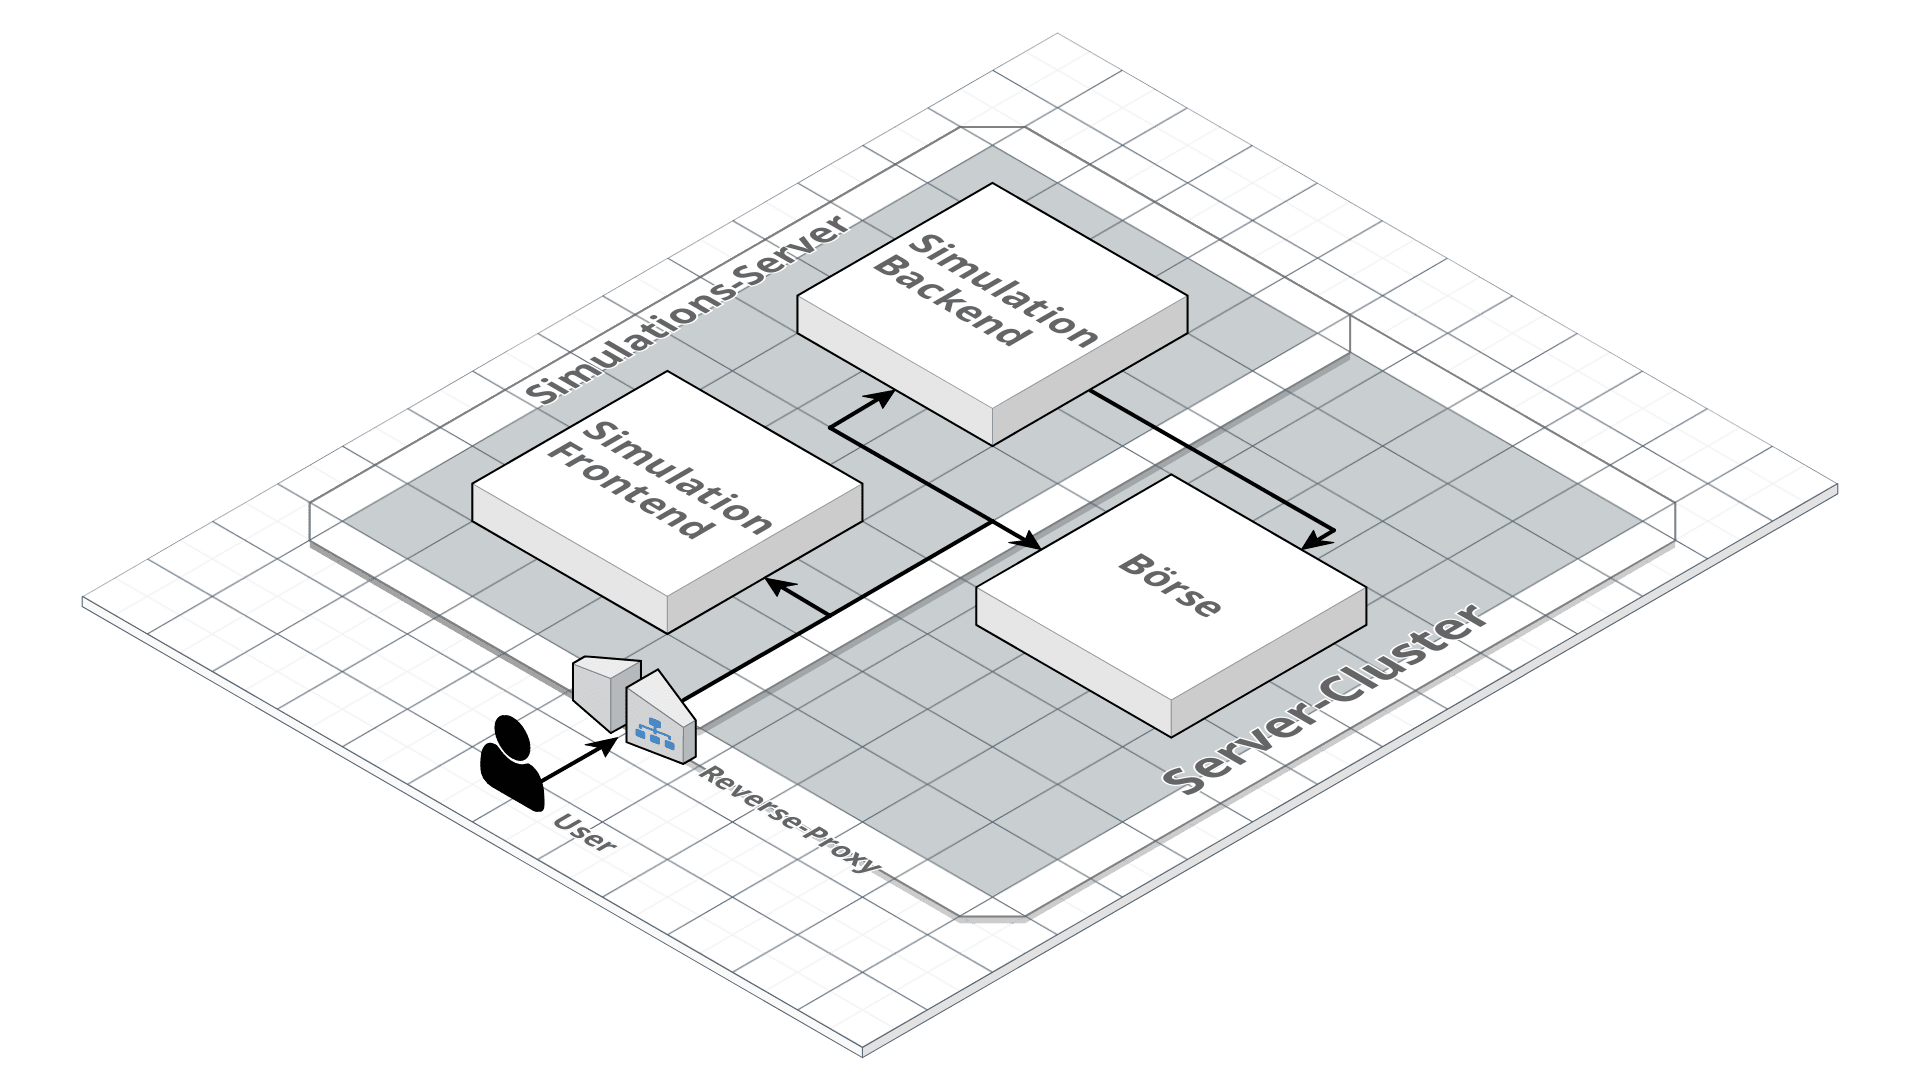
\includegraphics[width=\textwidth]{img/architecture.png}
    \centering
    \caption{Architektur}
    \label{fig:architecture}
\end{figure}

In \autoref{fig:architecture} ist die Architektur der Anwendung dargestellt.
Alle benötigten Server sind in einem Server-Cluster organisiert.
Hier werden die Börse, die Kernlogik der Simulation ausgeführt und das Nutzerinterface an den User ausgeliefert. Zentralles Eintrittstor ist dabei ein Reverse-Proxy, welcher die Aufgabe hat, die Daten an die richtigen internen Server weiterzuleiten und Daten, die für den Nutzer sind zu verschlüsseln.
Innerhalb des Clusters kommunizieren der Simulations-Backend-Server direkt mit der Börse. Dadurch kann dieser Verkehr nicht von außen beeinflusst werden und mögliche Aktieninformationen (beispielsweise welche Person welche Aktie handelt) sind geschützt.

Das Simulations-Frontend dient als grafische Benutzeroberfläche, mit dem das eigentliche Simulations-Backend gesteuert wird. Weitere Informationen dazu finden sich in \autoref{cha:Nutzerhandbuch}.

Unsere Architektur trennt dabei streng die Szenario-Logik vom Nutzerinterface.
Hat der Nutzer ein Szenario ausgewählt, alle Einstellungen getroffen und das Szenario gestartet, wird eine Anfrage an den Simulations-Backend-Server gesendet. Darauf hin beginnt dieser das entsprechende Szenario auszuführen und mit der Börse zu handeln.
Dies hat ein paar Vorteile gegenüber der Implementierung sämtlicher Logik innerhalb des Nutzerinterfaces:
\begin{enumerate}
    \item Zentrale Nutzersteuerung\\
        Der Backend-Server kann Ausführungen von Szenarien steuern. So werden beispielsweise Kollisionen vermieden, wenn mehrere Szenarien von verschiedenen Nutzern gestartet werden würden.
    \item Code-Qualität\\
        Durch die Trennung der Logik nach dem Separation-of-Concern und Clean-Code Methodiken wird der Quelltext wartbarer.
    \item Unterbrechungen\\
        Der Nutzer kann ein Szenario starten, welches eine längere Dauer hat (z.\,B. mehrere Tage). Anschließend muss er nicht seinen COmputer eingeschaltet lassen. Das Szenario wird im Hintergrund ausgeführt.
\end{enumerate}

\section{Szenario}
Wie in \autoref{sec:Architektur} beschrieben kümmert sich der Backend Server um die Ausführung der Szenarien.

Im Kern basiert die Szenarioausführung bildet auf einem Agenten-Ansatz. Agenten sind Computerelemente, die sich in bestimmten Umgebungen befinden und in der Lage sind eigenständige Entscheidungen zu treffen. Die Umgebung ist dabei der Aktienmarkt.
Da ein hoher Fokus auf eine realitätsnahe Simulation gelegt wird, orientiert sich die Implementierung dieser Agenten an einem Black-Box-Modell.
Wie in der Realität haben alle Agenten eigenständige Strategien und können sich jederzeit frei entscheiden wann welche Order erstellt wird. Dafür haben die Agenten ein eigenes, asynchrones Gehirn.
Weder andere Agenten noch der Server haben Informationen über das aktuelle Handeln eines einzelnen Agenden.

Sobald die Anfrage durch die \ac{API} im Server eingetroffen ist startet der Server direkt mit der Szenarioausführung. Dafür existiert ein Life-cycle, der mehrere Schritte nacheinander durchläuft (vergleiche \enquote{Endlicher Automat}):

\begin{enumerate}
    \item Server start\\
        Der Server wurde gestartet. Ab diesem Zeitpunkt kann der Server anfragen entgegen nehmen.
    \item Szenarios geladen\\
        Die Szenarios wurden aus den Quelldaten geladen und können nun gestartet werden.
    \item Szenario wird gestartet\\
        Über die \ac{API} wurde der Start eines Szenario angefordert und der Server initialisiert das Szenario.
        \begin{enumerate}
            \item Agenten Initialisierung\\
                Die Agenten werden erstellt und bekommen ihre Logik. Dafür werden neue Instanzen dieser Agenten erstellt. Zusätlich wird ihnen ein Verhalten zugewiesen, welches sie später ausführen sollen.
            \item Markt initialisierung\\
                Die Marktüberwachung wird gestartet, sodass die Agenten Informationen über den aktuellen Aktienpreis haben.
            \item Daten Initialisierung\\
                Die Agenten werden mit Daten, z.\,B. den Szenarieninformationen oder anderen Einstellungen befüllt.
                Möglich wäre hier auch eine Implementierung von existierenden Depots dieser Agenten.
            \item Agenten beleben\\
                Die Agenten werden belebt, sodass diese mit ihrer Logik beginnen und Orders erstellen.
        \end{enumerate}
    \item Szenario wird ausgeführt\\
        Das Szenario wird aktuell ausgeführt und die Agenten arbeiten.
    \item Szenario wird gestoppt\\
        Alle Agenten werden aufgefordert ihr Verhalten zu stoppen und das Szenario wird beendet.
\end{enumerate}


Da dieser Life-cycle bereits einige Schritte hat, ergibt sich eine erhöhte Komplexität, welches die Implementierung verlangsamen könnte.
Um dies vorzubeugen wurde der Code so gestaltet, dass es mit sehr geringem Aufwand möglich ist neue Verhalten für Agenten zu implementieren. So gibt es innerhalb des Quellcodes eine zentral Schnittstelle die eingebunden wird. Dies ist als eine abstrakte Klasse definiert. Sobald Entwickler diese benutzen, wird von der Entwicklungsumgebung bereits sämtlicher Code generiert. Zusätzlich ist diese Schnittstelle ausführlich innerhalb des Quellcodes dokumentiert, wodurch Entwickler bereits während des Entwickelns über IntelliSense ausführliche Informationen über die richtige Verwendung bekommen.


Für die Szenarioumsetzung ist primär das Szenario-Gehirn zuständig. Desen Entscheidungsprozess läuft kontinuierlich nach dem folgendem Muster ab:
\begin{enumerate}
    \item Daten finden\\
        Der Agent vergleicht die aktuell simulierte Zeit mit den Szenariendaten.
    \item Zielpreis ermitteln\\
        Konnte ein Datenpunkt identifiziert werden, wird der Zielpreis, welchen die Aktie annehmen, ermittelt. Dabei wird der aktuelle Marktpreis von der Börse mit dem Datenpunkt verrechnet.
    \item Matching Order erstellen\\
        Die in \autoref{sec:szenarien} beschriebenen Orders werden basierend auf dem Datenpunkt erstellt.
\end{enumerate}

\begin{figure}[ht]
    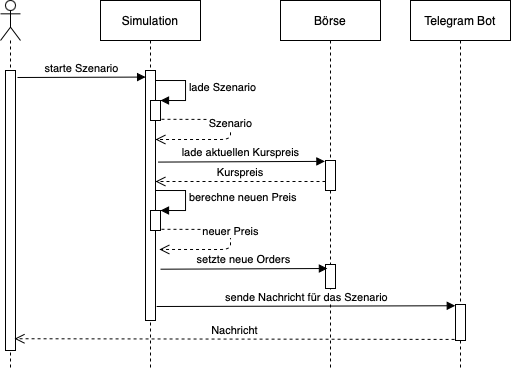
\includegraphics[width=\textwidth]{img/Sequenzdiagramm.png}
    \centering
    \caption{Sequenzdiagramm}
    \label{fig:Sequenzdiagramm}
\end{figure}


\section{User Interface}
//TODO: @aaron

% !TEX root =  ../master.tex
\chapter{Nutzerhandbuch}
% Fazit und Ausblick
% !TEX root =  master.tex
\chapter{Zusammenfassung}

In der vorliegenden Arbeit haben wir uns damit auseinander gesetzt, wie sich Börsenverläufe simulieren lassen können. Dabei wurden sowohl komplexe Algorithmen als auch simplere betrachtet und auf ihre Anwendbarkeit auf die gegebene Aufgabenstellung bewertet. Nach diesem Einarbeitung und Auseinandersetzung Schritt, wurde ein Tool entwickelt und umgesetzt, dass einen solchen Algorithmus implementiert und das Handeln an einer Börse unter Markt ähnlichen Bedingungen ermöglicht. Dabei sei darauf hinzuweisen, dass wir den Anwendungsfall hauptsächlich für Bildungszwecke sehen. Zwar orientieren sich die enthaltenen Szenarien an echten Börsenverläufen, jedoch sind reale Börsenzusammenhänge sehr komplex und die Marktsituationen heute können sich von den von uns gewählten historischen Situationen unterscheiden. Eine in der Simulation gut funktionierende Strategie muss daher nicht zwingend auf einem realen Markt funktionieren. Außerdem distanzieren wir uns von sämtlichen Anlageberaterischen Tätigkeiten. Zweck der Anwendung ist ausschließlich das spielerische erlangen eines besseren Verständnisses über den Aktienmarkt und unterschiedliche Strategien. Dabei ermöglichen wir eine risikofreie Testung von unterschiedlichen Strategien und Ansätzen, da die durch die Simulation durchgeführten Transaktionen keinen Bezug zu realen Währungen und den damit verbundenen finanziellen Verlusten haben. 

\section{Fazit}
Insgesamt sind wir mit der Ausarbeitung und der Arbeit innerhalb unserer Teilgruppe sehr zufrieden. Dennoch hat das Projekt auch bei uns einige Learnings hervorgebracht. Diese liegen im wesentlichen in der Teamübergreifenden Arbeit und dem Projektgeschehen. 

	\begin{itemize}
		\item Früher POCs und MVPs nutzen: \\
			Dies hätte uns ev. die Mehraufwände und Einschränkungen durch die Performance und Lastprobleme zwischen der Simulation und der Börse erspart, die sich auch auf die anderen Broker ausgewirkt hat. 
		\item Effektivere Kommunikation in den Abstimmungsmeetings (Agenda, o.Ä)
		\item Klarere Aufgabendefinitionen: \\
			Hätte zumindest in unserer Gruppe dazu geführt Aufwände bei der theoretischen Einarbeitung und Implementierungen zu reduzieren, da
		\item Früher Feedback vom Kunden: \\
			Auch hier hätte uns schnelleres Feedback unter Umständen Aufwände ersparen können und einen noch größeren Mehrwert für das gesamte Projekt in der selben Zeit generiert werden können. 
		\item Definierte Ansprechpartner im Fehlerfall
		
	\end{itemize}

In der von uns entwickelten Anwendung sehen wir vor allem den Vorteil, dass diese sehr skalierbar ist. So können einfach weitere Aktien hinzugefügt und simuliert werden. Auch das ergänzen von weiteren Szenarien ist ohne weitere Implementierungsaufgaben möglich. Außerdem kann unsere Anwendung auch mit höheren Frequenzen, also mehr Trades pro Sekunde und deutlich größeren Volumina arbeiten.  
%%%%%%%%%%%%%%%%%%%%%%%%%%%%%%%%%%%

\initializeAppendix

%%%%%%%%%%%%%%%%%%%%%%%%%%%%%%%%%%%
% ANHÄNGE
%
% @stud: einzelne Anhänge bearbeiten und eigene Anhänge hier einfügen 
%
% % !TEX root =  master.tex
\chapter{Beispiel-Anhang: Testanhang}
Anh\"ange\index{Anhang} werden am Ende Ihrer Arbeit vor dem Literaturverzeichnis und dem Index eingef\"ugt.

\section{Abschnitt im Anhang}

\lipsum

%%%%%%%%%%%%%%%%%%%%%%%%%%%%%%%%%%%

\singlespacing

%%%%%%%%%%%%%%%%%%%%%%%%%%%%%%%%%%%
% LITERATURVERZEICHNIS
% 
% @stud: Literaturverzeichnis in Datei bibliography.bib anpassen 
%
\initializeBibliography
%%%%%%%%%%%%%%%%%%%%%%%%%%%%%%%%%%%

\addcontentsline{toc}{chapter}{Index}
\printindex

\end{document}
